\documentclass[a4paper,DIV=12]{scrartcl}
\usepackage[utf8]{inputenc}

\usepackage[T1]{fontenc}
\usepackage{tgtermes}
\usepackage{tgheros}
\usepackage{tgcursor}
\usepackage[english]{babel}

\usepackage{graphicx}
\usepackage{listings}
\usepackage{microtype}
\usepackage{xcolor}

\title{Pyramid}
\subtitle{Exercise for learning to program scripts for PADrend}
\author{Benjamin Eikel \and Claudius Jähn}

\begin{document}
\lstdefinelanguage{EScript}{
	morekeywords={var,new,fn,this,true,false,void,if,else,while,for,foreach,as,thisFn,break,continue,return},
	morekeywords=[2]{out,ExtObject,Type,Number},
	morekeywords=[3]{MinSG, PADrend},
	sensitive=true,
	morecomment=[l]{//},
	morecomment=[s]{/*}{*/},
	morestring=[b]{"},
	morestring=[d]{’}
}
\lstset{
	language=EScript,
	showstringspaces=false,
	tabsize=4,
	basicstyle=\small\ttfamily,
	keywordstyle=[2]\color{blue},
	keywordstyle=[3]\color{teal},
}
\maketitle
\section*{Introduction}
\begin{figure}[htbp]
	\centering
	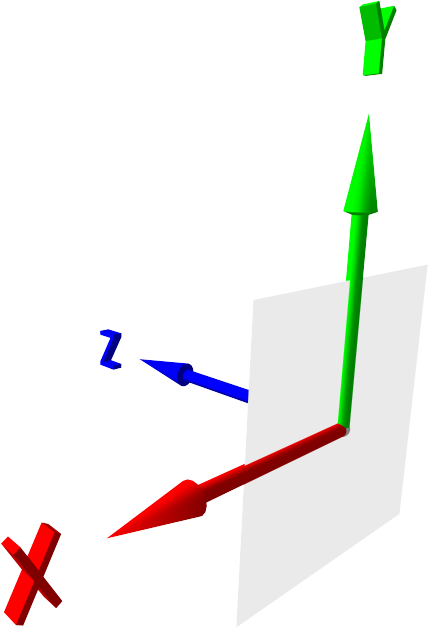
\includegraphics[width=4cm]{rectangle}
	\caption{Rectangle with coordinate system}
	\label{fig:rectangle}
\end{figure}
Given is the \lstinline!Mesh! of a rectangle, which has a size of one times one units.

A mesh is an array of vertices, an array of indices, and the description of the attributes of the vertices.
A vertex is defined by its index inside the array and stores the values of its attributes.
Commonly used attributes are a three-dimensional position vector, a three-dimensional normal vector, an RGB color value, and a two-dimensional texture coordinate.
The second array of the mesh stores the indices that compose a primitive.
For example, if the mesh is used to store triangles, every three indices compose a triangle.
In MinSG, to store a mesh inside the scene graph, the mesh is attached to a \lstinline!GeometryNode!.

Figure~\ref{fig:rectangle} shows the rectangle together with a coordinate system.
The coordinate system visualizes the placement of the rectangle inside the world coordinate system.
The rectanlge lies inside the x-y plane with its center being the origin.

The following script creates the rectangle and attaches it to a node.
\lstinputlisting[firstline=3, lastline=6]{exercise1_solution.escript}

To create a new root node for a scene, an instance of a \lstinline!ListNode! is created:
\lstinputlisting[firstline=8, lastline=8]{exercise1_solution.escript}

A \lstinline!ListNode! groups multiple nodes -- its children -- together.
To tell PADrend to use a node as the current scene, the node has to be registered as a scene and selected:
\lstinputlisting[firstline=49, lastline=50]{exercise1_solution.escript}
\section*{Exercise 1}
\begin{figure}[htbp]
	\centering
	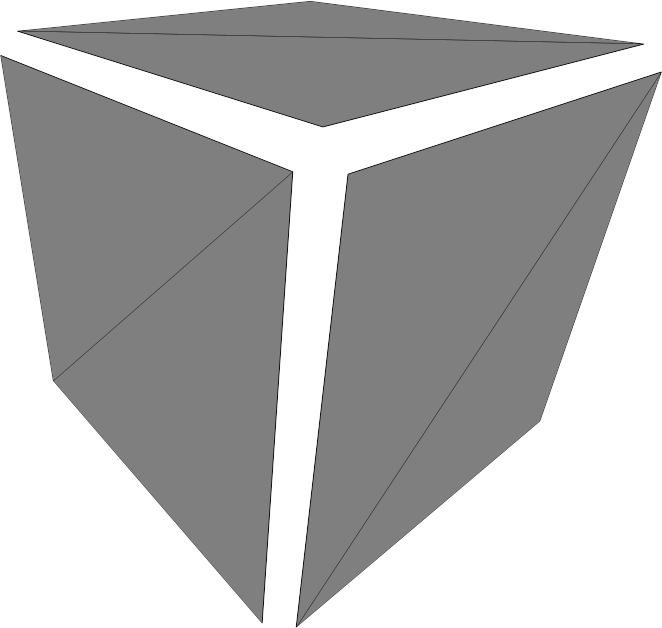
\includegraphics[width=4cm]{cube}
	\caption{Exploded view of a cube, which is composed of multiple rectangles}
	\label{fig:cube}
\end{figure}
Use the given rectangle six times to create a cube.
Rotate and translate the rectangles into the correct position.
The cube should look like the one in Figure~\ref{fig:cube}.
The following script shows an example on how to create and transform a single side.
\lstinputlisting[linerange={10-11,22-29,46-47}]{exercise1_solution.escript}
\section*{Exercise 2}
\begin{figure}[htbp]
	\centering
	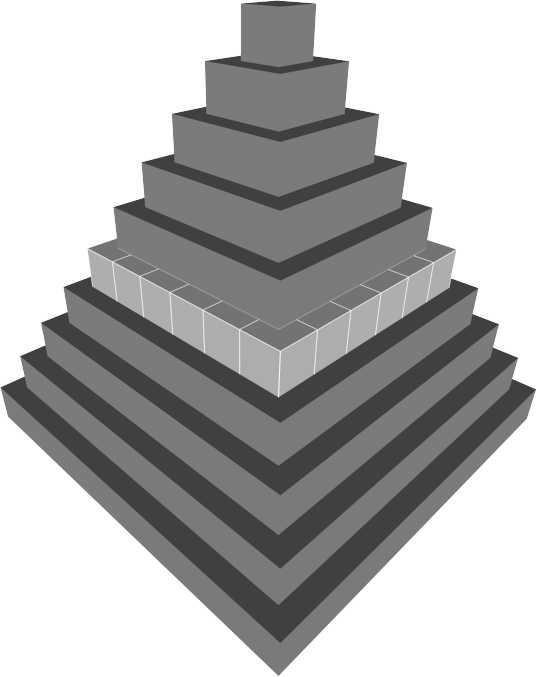
\includegraphics[width=4cm]{pyramid_gray}
	\caption{A pyramid with ten levels composed of cubes}
	\label{fig:pyramid_gray}
\end{figure}
Build a pyramid of cubes.
You can reuse the cube node from the previous exercise.
Use a scene graph structure, such that every level of the pyramid is a group.
An example of a pyramid can be seen in Figure~\ref{fig:pyramid_gray}.
\section*{Exercise 3}
\begin{figure}[htbp]
	\centering
	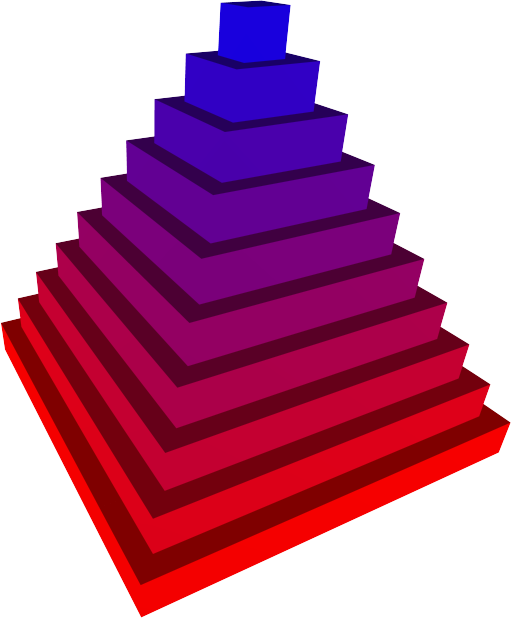
\includegraphics[width=4cm]{pyramid_colored}
	\caption{A pyramid with a different color for each level}
	\label{fig:pyramid_colored}
\end{figure}
Color the pyramid from the previous exercise with a gradient.
The top level should be colored red.
The bottom level should be colored blue.
For each level, only a single material should be used.
In MinSG, a material can be added to a node by attaching a \lstinline!MaterialState! to the node.
The material is defined by an ambient color, a diffuse color, a specular color, and a shininess coefficient.
\begin{lstlisting}
var materialState = new MinSG.MaterialState();
// Color values are from the interval [0.0, 1.0]
var color = new Util.Color4f(red, green, blue, alpha);
materialState.setAmbient(color);
materialState.setDiffuse(color);
node.addState(materialState);
\end{lstlisting}
The final pyramid could look like the one shown in Figure~\ref{fig:pyramid_colored}.

\section*{General Hints}
To execute a script inside PADrend, a very simple way is to store the script file in the \texttt{presets} directory in PADrend's main directory and then select it in PADrend using the SpeedDial-plugin (press \texttt{[F3]}).
The script is evaluated whenever the button is pressed, so there is no need to restart PADrend after you changed the script.

To execute a single line of code, you can use the Console plugin (press \texttt{[\^{}]}), which is bundled with PADrend.
For example, to output information for the available attributes of a \lstinline!MaterialState!, enter \lstinline!info(MinSG.MaterialState);! and press "execute".

\end{document}
